\subsection{Introduction}
\label{subsec:introduction2}
A Tensor Processing Unit (TPU), similar to a Graphical Processing Unit (GPU) and Central Processing Unit (CPU), is a computing device with the difference being the focus of their activities.
While GPUs and CPUs are considered general purpose, TPUs are a special purpose; they are built to speed up the performance of ML related applications, particularly in linear algebraic processes involving matrices.
They cannot do much else, at least not efficiently.
As of now, the TPU has iterated to its fifth version, but for the purposes of this work, we will mention only TPUv4 and highlight the important features it has.

\subsection{Structure}
\label{subsec:structure}
There are 2 main components of a TPU chip: High Bandwidth Memory (HBM) and the Tensor Cores (TC).
The HBM is an on-chip memory allowing for larger models and bigger batch sizes.
The TCs on the other hand consist of many multiply-accumulators; the special hardware that allows for an increase in speed for matrix-related operations.
These multiply-accumulators are all arranged in an array-like structure called the systolic array structure.

Google’s TPU machine consists of thousands of these TPU chips (as of TPUv4, there are 4096 chips placed inside).
Within the machine itself, the chips are arranged physically as a cube, but the inner networking between the chips would form a torus.
This is actually only the default configuration.
Users are able to define their own topology (in terms of networking).

The TPU works by first loading parameters from the HBM, load them into individual multiply-accumulators and then load the data to one layer of the array-like architecture and let the results of one computation feed the next one, and so on.
It is akin to how a ripple-carry adder works.

\subsection{TPUv4}
\label{subsec:tpuv4}
These features are all common amongst the different iterations of the TPU\@.
If so, then what is so important about the TPUv4?
The main improvements introduced handles around the subject of scale and reliability using google's very own advancement in optical switches.
Additionally, just as any other kind of iteration, the TPUv4 also improves certain aspects of the system, i.e.,\ on the dealing with storage of embeddings by introducing the appropriate hardware architectures and introducing a way that allows for a better compatibility between hardware and the model.

\subsubsection{Reconfigurable Optical Switches}
As mentioned, the TPUv4 has 4096 TPU chips.
This number may seem insignificant to some, but we can compare that to the previous version’s (TPUv3) 1024 chips.
The sheer size of the TPUv4 renders electrical switches useless due to “electrical interconnect” limitations.
To solve this, optical switches were used.
In particular, Google's Palomar Optically Configurable Switches (OCS).
They are based on Micro-Electro-Mechanical Systems that can send light both ways in a fiber by employing what is called a ``circulator``.

\begin{figure}[htbp!]
    \centerline{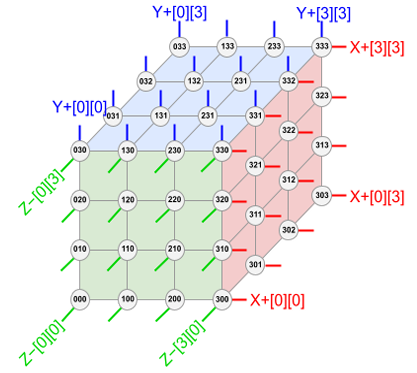
\includegraphics[width=0.2\textwidth]{images/tpu_cube}
    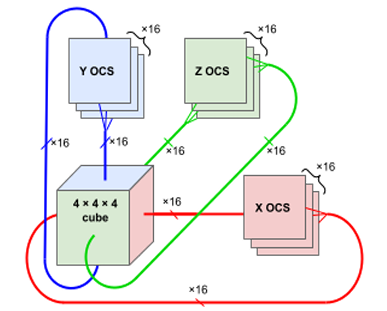
\includegraphics[width=0.2\textwidth]{images/tpu_connectivity}}
    \caption{OCS Architecture.}
    \label{fig:ocsarch}
\end{figure}

The figure illustrates how the OCSs are connected.
This cube, a 4 x 4 x 4, is part of the TPU machine that consists of many TPU chips that must be connected to the OCS (We consider a cubic arrangement of 64 chips due to nicer bisection bandwidth and for convenience in storage).
The way we connect them is by connecting each side’s chips to the OCS and the opposite side of that side connected to the same OCS\@.
In total, for TPUv4, there are typically 3 * 16 = 48 OCSs for a single machine.

The OCS brings a multitude of benefits.
The first is availability and deployment benefits.
Being flexible and having better performance allows TPUv4 to still provide good services, although some hosts of the system may not be available.
And because the OCSs bring some sort of independence to the system (particularly, it made each rack of the chips more independent), not all chips are needed to ensure operability.

Then, the most obvious one, configurable.
The OCS greatly simplifies scheduling and networking within the system due to its great switching speed.
For instance, it no longer has to search for many contiguous chips during scheduling, and it allows modularity between users (the whole system can cater to multiple users) which enhances security.
Finally, foreshadowed before, the whole system can be reconfigured to one's topological needs, like exploiting parallelisms, as ``rewiring`` the system mostly involves reprogramming the routes of the OCS\@.

\subsubsection{SparseCore}
Like any other computers dealing with ML, This one is for dealing with embedding.
In particular, where to store the lookup tables from the embedding process.
The main problem here is that the lookup operations will cause a bottleneck for the chips due to memory accesses, inter-chip communication, etc.
As they are more suited for dense arithmetic operation.

In this context, there were two possible solutions: either put it in the host’s CPU or put it in the tensor cores themselves.
The Host’s CPU approach would introduce a bottleneck during the next iterations of Amdahl’s law; in comparison, there is a 4:1 TPUv4 to host CPU ratio.
On the other hand, putting it in the TC would be suboptimal due to their nature.
A way out of this is to use both the HBM and the dedicated Inter-Core Interconnect (ICI) network which are embedded in the chips.
With these in mind, comes SparseCore (SC).
It is an additional hardware put in the machine for dealing with embedding training.
SC uses the HBM and a dedicated ICI network while operating in a sea of cores configuration creating a flat, globally addressable memory space.

\subsubsection{Platform-Aware Neural Architecture Search}
Platform-Aware Neural Architecture Search or PA-NAS has a goal to configure both the ML model and the TPU topology to benefit from each other as much as possible.
In particular, with the mention of SC, a model in the TPU might need to use both SC and TC efficiently.
PA-NAS optimizes operations related to this to achieve ``pareto-optimal performance and quality``.